\documentclass{article}
\usepackage[top=2.5cm, bottom=2cm, left=3cm, right=2cm]{geometry}
\usepackage[utf8]{inputenc}
\usepackage{amsthm}
%\usepackage[]{babel}
\usepackage{amssymb}
\usepackage{amsmath}
\usepackage{graphicx}
\usepackage{bm}
\usepackage{listings}
\usepackage{indentfirst}
%\usepackage{hyperref}

\newtheorem{theorem}{Theorem}[section]
\newtheorem{corollary}{Corollary}[theorem]
\newtheorem{lemma}[theorem]{Lemma}

\renewcommand\qedsymbol{$\blacksquare$}

\renewcommand{\contentsname}{\center{Sumário}}
%%%%%%%%%%%%%%%%%%%%%%%%%%%%%%%%%%%% Python Codes %%%%%%%%%%%%%%%%%%%%%%%%%%%%%%%%%%%%%%%%%%%%%%%%%%%%%%%%%%%%%%%%%%%%%%%%%%

% Default fixed font does not support bold face
\DeclareFixedFont{\ttb}{T1}{txtt}{bx}{n}{10} % for bold
\DeclareFixedFont{\ttm}{T1}{txtt}{m}{n}{10}  % for normal

% Custom colors
\usepackage{color}
\definecolor{deepblue}{rgb}{0,0,0.5}
\definecolor{deepred}{rgb}{0.6,0,0}
\definecolor{deepgreen}{rgb}{0,0.5,0}

% Python style for highlighting
\newcommand\pythonstyle{\lstset{
language=Python,
basicstyle=\ttm,
otherkeywords={self},             % Add keywords here
keywordstyle=\ttb\color{deepblue},
emph={MyClass,__init__},          % Custom highlighting
emphstyle=\ttb\color{deepred},    % Custom highlighting style
stringstyle=\color{deepgreen},
frame=tb,                         % Any extra options here
showstringspaces=false            % 
}}

% Python environment
\lstnewenvironment{python}[1][]
{
\pythonstyle
\lstset{#1}
}
{}

% Python for external files
\newcommand\pythonexternal[2][]{{
\pythonstyle
\lstinputlisting[#1]{#2}}}

% Python for inline
\newcommand\pythoninline[1]{{\pythonstyle\lstinline!#1!}}

%%%%%%%%%%%%%%%%%%%%%%%%%%%%%%%%%%%%%%%%%%%%%%%%%%%%%%%%%%%%%%%%%%%%%%%%%%%%%%%%%%%%%%%%%%%%%%%%%%%%%%%%%%%%%%%%%%%%%%%%%%%%

\begin{document}

\theoremstyle{definition}
\newtheorem{definition}{Definition}[section]

\begin{center}

FIS0610 - Física Computacional I

\vspace{1em}
{\Huge Uma Breve Introdução ao Python\footnote{Python 2.7.12}}

\vspace{1em}
Paulo Douglas Santos de Lima\\
\texttt{paulo.douglas.lima@fisica.ufrn.br}\\

\end{center}

\tableofcontents

\newpage

\section{Problema 1}


\section{Problema 2}

\section{Problema 3}
 O gráfico com as quantidades $y_1$, $y_2$ e $y_3$ está apresentado na figura 1 com seu código abaixo. Note que para evitar divisões por 0, os valores de $E$ foram iniciados em 0.1.
\pythonexternal{q3a_l4.py}
\begin{center}
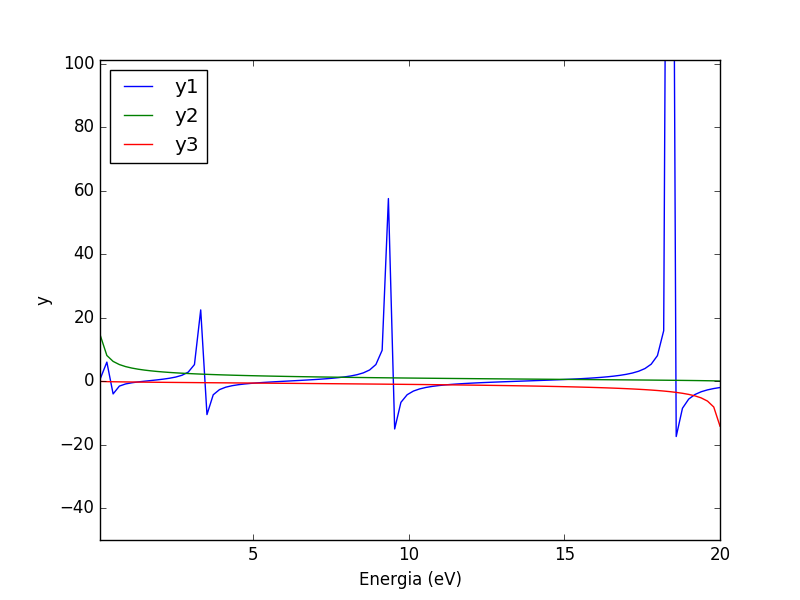
\includegraphics[scale=0.75]{ex3a}
\end{center}
 
 Analisando cuidadosamente o gráfico e evitando os pontos de singularidades da função tangente, obtemos uma estimativa dos primeiros seis níveis de energia:
	\begin{table}[h]
    		\centering
        \caption{Valores estimados para os seis primeiros níveis de energia.}
        \label{tab:expcond}
        \begin{tabular}{c|c}
            Níveis Pares (eV) & Níveis Ímpares (eV) \\
            \hline
            0,318 & 1,255 \\
            2,850 & 5,125 \\
            7,875 & 11,45 	\\
        \end{tabular}
    \end{table}

 Na luz desses valores, o algoritmo abaixo foi desenvolvido para o cálculo das raízes usando o método da bisecção com intervalos adequados. O valor máximo usado de erro para a raiz foi de 0.001 e o número de interações foi calculado com base na inequação:
 
 \begin{equation}
 	n_{max} \geq \frac{\log(b-a) - \log(2\epsilon)}{\log(2)}\,,
 \end{equation}
 que garante a convergência do método após $n_{max} + 1$ iterações.

\pythonexternal{q3_l4.py}
 
\section{Problema 4}
 O algoritmo para a construção do polinômio de Legendre e o gráfico estão abaixo:
 \pythonexternal{q4_l4.py}
 	\begin{center}
		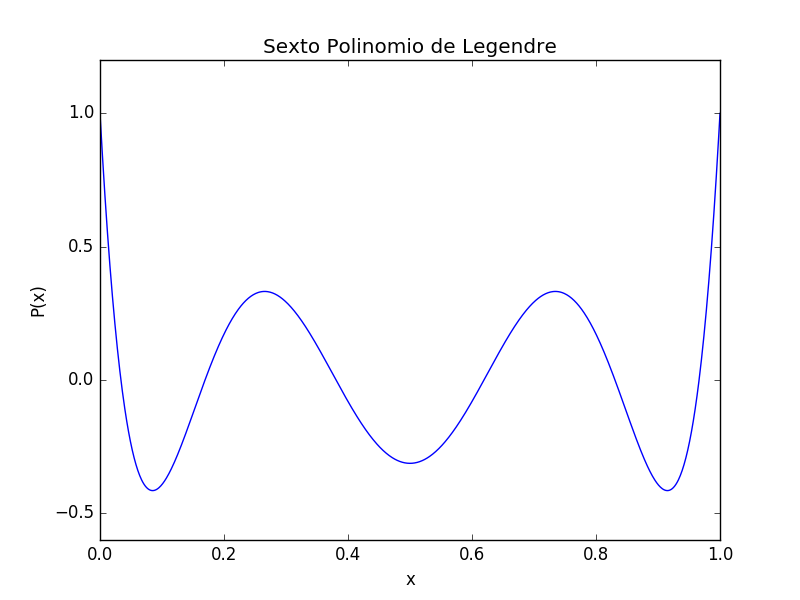
\includegraphics[scale=0.75]{ex4}
	\end{center}
 \newpage
  
 Para determinar as raízes utilizando o método de Newton, foi utilizado a biblioteca \emph{scipy.optmize\footnote{https://docs.scipy.org/doc/scipy/reference/generated/scipy.optimize.newton.html}}, que já implementa internamente este método. O ponto inicial usado foi o estimado pela análise gráfica, enquanto que a tolerância para os valores das raízes de $10^{-10}$, que levou ao número de 800 iterações.
\pythonexternal{ex4.py}
\begin{table}[h]
    		\centering
        \caption{Comparação entre o valor das raízes estimadas e numéricas.}
        \label{tab:expcond}
        \begin{tabular}{l|l}
            Raíz Estimada & Raiz Calculada Numericamente \\
            \hline
            0.035 & 0.0337652428984\\
		    0.168 & 0.169395306767 \\
			0.382 & 0.38069040712  \\
			0.618 & 0.380690407087 \\
			0.832 & 0.83060469899  \\
			0.967 & 0.0337652428984
        \end{tabular}
    \end{table} 

\section{Problema 5}


\end{document}








\grid
